\documentclass[times,twocolumn,final]{elsarticle}
%% Stylefile to load PR Letters template
\usepackage{prletters}
\usepackage{framed,multirow}
\usepackage{algorithm}
\usepackage{algpseudocode}
%% The amssymb package provides various useful mathematical symbols
\usepackage{amssymb}
\usepackage{latexsym}
\usepackage{url}
\usepackage{amsfonts} 
\usepackage{amsmath}
\usepackage{amsthm}
\usepackage{pifont}
\usepackage{natbib}
\usepackage{geometry}
\usepackage{graphicx}
\usepackage{color} 
 
\newcommand{\subfigimg}[3][,]{%
  \setbox1=\hbox{\includegraphics[#1]{#3}}% Store image in box
  \leavevmode\rlap{\usebox1}% Print image
  \rlap{\hspace*{12pt}\raisebox{\dimexpr\ht1-0\baselineskip}{#2}}% Print label
  \phantom{\usebox1}% Insert appropriate spcing
}
%ming's package for numerical section 
\RequirePackage{lineno}
\usepackage{subfig}
%\usepackage{setspace}

\newenvironment{Table}
  {\par\bigskip\noindent\minipage{\columnwidth}\centering}
  {\endminipage\par\bigskip}
	
%flowchart
\usepackage{tikz}
\usetikzlibrary{shapes.geometric, arrows}
\tikzstyle{node} = [rectangle, rounded corners, minimum width=0.5cm, minimum height=0.5cm,text centered, draw=black, fill=white!30]
\tikzstyle{arrow} = [thick,->,>=stealth]

\newcommand{\jv}[1]{{\color{magenta}{\it #1}}}
\newcommand{\cs}[1]{{\color{blue}{\it #1}}}
\newcommand{\Linefor}[2]{%
    \State \algorithmicfor\ {#1}\ \algorithmicdo\ {#2} \algorithmicend\ \algorithmicfor%
}
\newcommand{\Lineif}[2]{%
    \State \algorithmicif\ {#1}\ \algorithmicdo\ {#2} \algorithmicend\ \algorithmicif%
}
\newcommand{\rto}{\leftarrow}
\providecommand{\mb}[1]{\boldsymbol{#1}}

\begin{document}

\begin{frontmatter}
\title{Manifold Matching using Shortest-Path Distance and Joint Neighborhood Selection}
\author[1,2]{Cencheng Shen}
\ead{cshen6@jhu.edu}
\author[2,3]{Joshua T. Vogelstein}
\ead{jovo@jhu.edu}
\author[2,4]{Carey E. Priebe\corref{cor1}}
\ead{cep@jhu.edu}

\address[1]{Department of Statistics, Temple University}
\address[2]{Center for Imaging Science, Johns Hopkins University}
\address[3]{Department of Biomedical Engineering and Institute for Computational Medicine, Johns Hopkins University}
\address[4]{Department of Applied Mathematics and Statistics, Johns Hopkins University}
\cortext[cor1]{Corresponding author}

\begin{abstract}
Exploring and matching datasets of multiple modalities has become an important task in data analysis. Most existing matching methods rely on embedding and transformation techniques for dataset of a single modality without fully utilizing the correspondence information, which often yields sub-optimal matching results. In this paper we propose a new nonlinear manifold matching algorithm using shortest-path distance and joint neighborhood selection. Specifically, a joint graph is built for all modalities. Then the shortest-path distance within each modality is calculated from the joint neighborhood graph, followed by embedding into and matching in a common low-dimensional Euclidean space. Compared to existing popular algorithms, our approach exhibits superior performance for matching disparate datasets of multiple modalities. 
\end{abstract}
\begin{keyword}
manifold matching, shortest-path distance, joint neighborhood selection
\end{keyword}
\end{frontmatter}

\section{Introduction}
In today's world, it is becoming increasingly important to deal effectively with large amounts of high-dimensional data. For the purpose of data analysis, it is imperative to consider dimension reduction and embed the data into a low-dimensional space for subsequent analysis. Traditional linear embedding techniques have solid theoretical foundations and are widely used. For example, principal component analysis (PCA) \citep{JolliffePCABook, BishopTipping1999} and multidimensional scaling (MDS) \citep{TorgersonBook, BorgBook, CoxBook} for dataset of a single modality, and canonical correlation analysis (CCA) \citep{Hotelling1936, BachJordan2005} for datasets of multiple modalities. 

However, real datasets may exhibit nonlinear geometry, and discovering the underlying non-linearity can be beneficial for subsequent inference. Many manifold learning algorithms have been proposed to learn the intrinsic low-dimensional structure of nonlinear dataset, including Isomap \citep{TenenbaumSilvaLangford2000, SilvaTenenbaum2003}, locally linear embedding (LLE) \citep{SaulRoweis2000, RoweisSaul2003}, Hessian LLE \citep{DonohoGrimes2003}, Laplacian eigenmaps \citep{BelkinNiyogi2003, HeEtAl2005}, local tangent space alignment (LTSA) \citep{ZhangZha2004, ZhangWangZha2012}, among many others. %Most of them start with the assumption that the data are locally linear, explore the local geometry via the nearest-neighbor graph of the sample data, carry out transformation of the data based on the neighborhood graph, and eventually learn the low-dimensional manifold by optimizing some objective function. 
These nonlinear embedding algorithms usually serve as a preliminary feature extraction step that enables subsequent inference. They have been used successfully in object recognition and image processing. 

In this paper, we consider the manifold matching task for datasets of multiple modalities. Classical methods for identifying the relationship among multiple random variables are still very popular in theory and practice, such as canonical correlation \citep{Hotelling1936, Kettenring1971, Hardoon2004} and Procrustes transformation \citep{Sibson1978, Sibson1979, GoldbergRitov2009, GowerProcrustesBook}. However, it has become a much more challenging task to match real datasets of multiple modalities from disparate sources, such as the same document in different languages, an image and its descriptions, or networks of the same actors on different social websites. 

There have been many recent endeavors regarding data fusion and manifold matching \citep{LafonKellerCoifman2006, WangMahadevan2008, WangMahadevan2012, SharmaKumar2012, PriebeMarchette2012, SunPriebeTang2013, ShenSunTangPriebe2014}. Similar to dimension reduction for dataset of a single modality, manifold matching can serve as a feature extraction step to explore datasets of multiple modalities, and has also been shown to help subsequent inference in object recognition \citep{KimKittlerCipolla2007}, information retrieval \citep{SunPriebe2012}, and transfer learning \citep{PanYang2010}. Furthermore, the matching task is important on its own and has been applied to explore multiple graphs and networks \citep{LyzinskiFishkindPriebe2014, JoshuaEtAl2015, LyzinskiFishkindPriebe2016}. One such application is seeded graph matching, where two large networks are collected but only a percentage of training vertices have known correspondence. Thus, the remaining vertices need to be matched properly to uncover the potential correspondence.

Due to the success of nonlinear embedding algorithms for dataset of a single modality, it is often perceived that these algorithms can be combined into the matching framework to improve the matching performance when one or more modalities are nonlinear. A na\"ive procedure is to pick one nonlinear algorithm, apply it to each modality separately, and match the embedded modalities. But such a simplistic procedure does not always guarantee a good matching performance, since many nonlinear embedding algorithms only preserve the local geometry up to some affine transformation \citep{GoldbergRitov2008}. Furthermore, we will show in the numerical experiments that a direct matching of separate nonlinear embeddings can even deteriorate the matching performance when compared to linear embeddings.

To tackle the problem, we propose a manifold matching algorithm using shortest-path distance and joint neighborhood selection. By utilizing a robust distance measure that approximates the geodesic distance, and effectively combining the correspondence information into the embedding step, our proposed algorithm can significantly improve the matching quality from disparate data sources, compared to matching linear embeddings or separate nonlinear embeddings. All codes and data are available on our website \footnote{\url{https://github.com/cshen6/MMSJ}}.%Furthermore, the improvement in manifold matching motivates our follow-up work \citep{ShenEtAl2016} regarding dependency discovery by local scale, which makes use of the joint neighborhood in a different manner.

%The paper is organized as follows: In Section~\ref{bg} we describe the matching task and the evaluation criteria in mathematical notations. The proposed nonlinear manifold matching algorithm is presented in Section~\ref{main1}, with various implementation issues discussed in Section~\ref{discuss}. In Section~\ref{numer}, we illustrate the advantages of our algorithm via numerical simulations and real data experiments, using the simulated Swiss roll simulation and the Wikipedia document datasets with text and graph features. Finally, we summarize the results in Section~\ref{conclu}. All codes and data are available on our website \footnote{\url{https://github.com/cshen6/MMSJ}}.

\section{Manifold Matching}
\label{main}

\subsection{The Matching Framework}
\label{bg}
Suppose $n$ objects are measured under two different sources. Then $X_{l}=\{x_{il}\} \in \Xi_{l}$ for $l=1, 2$ are the actual datasets that are observed / collected, with $x_{i1} \sim x_{i2}$ for each $i$ ($\sim$ means the two observations are matched in the context). Thus $X_{1}$ and $X_{2}$ are the two different views / modalities of the same underlying data. This setting is extendable to datasets of more than two modalities, but for ease of presentation we focus mainly on the matching task of two modalities.

$\Xi_{1}$ and $\Xi_{2}$ are potentially very different from each other, such as a flat manifold and its nonlinear transformation, an image and its description, or texts under different languages. We assume $x_{il} \in \Xi_{l}$ is endowed with a distance measure $\Delta_{l}$ such that $\Delta_{l}(i,j)=dist(x_{il},x_{jl})$. To match multiple modalities, we find two mappings $\rho_{l}: \Xi_{l} \rightarrow \mathbb{R}^{d}, l=1,2$ such that the mapped data $\hat{X}_{l}=\{ \rho_{l}(x_{il}) \}$ are matched into a common low-dimensional Euclidean space $\mathbb{R}^{d}$. A simple example of $\rho_{l}$ can be MDS or PCA followed by CCA, which is a linear embedding and matching procedure.

Once the mappings are learned, for any new observations $y_{1} \in \Xi_{1}$ and $y_{2} \in \Xi_{2}$ of unknown correspondence, the learned mappings $\rho_{l}$ can be applied to match the testing observations in the low-dimensional Euclidean space, i.e., $\hat{y}_{l} = \rho_{l}(y_{l}) \in \mathbb{R}^{d}$. Ideally, a good matching procedure should be able to correctly identify the correspondence of the new observations, i.e., if the testing observations are truly matched in the context, the mapped points should be very close to each other in the common Euclidean space. If the testing observations are not matched, the mapped points should be far away from each other.

To evaluate a given matching algorithm, a natural criterion is the matching ratio used in seeded graph matching \citep{LyzinskiFishkindPriebe2014}. Suppose sufficient training observations are given to learn the mappings, and there exist some testing observations of unknown correspondence in each space. Assume that for each testing observation $y_{1}$ in $\Xi_{1}$, there is another testing observation $y_{2} \in \Xi_{2}$ such that $y_{1} \sim y_{2}$. Then they are correctly matched if and only if $\hat{y}_{2}$ is the nearest neighbor of $\hat{y}_{1}$ among all mapped testing data from $\Xi_{2}$. The matching ratio represents the percentage of correct matching of all testing observations, and thus a higher ratio indicates a better matching algorithm. 

The matching ratio based on nearest neighbor is often conservative, and can be a very small number when matching disparate real datasets. In practice, it is often more interesting to consider all neighbors within a small threshold, or rank multiple neighbors up to a limit. To that end, the statistical testing power of the hypothesis $H_{0}: y_{1} \sim y_{2}$ considered in \citep{PriebeMarchette2012} is another suitable criterion, which takes the Euclidean distance $\|\hat{y}_{1}- \hat{y}_{2}\|$ as the test statistic. To estimate the testing power for given data, we first split all observations into matched training data pairs, matched testing data pairs, and unmatched testing data pairs. After learning $\rho_{l}$ from the matched training data and applying them to all testing data, the test statistic under the null hypothesis can be estimated from the matched testing pairs, and the test statistic under the alternative hypothesis can be estimated from the unmatched testing pairs. The testing power at any type $1$ error level is directly estimated from the empirical distributions of the test statistic, and a higher testing power indicates a better manifold matching algorithm. 

We use both the testing power and the matching ratio for evaluation in the numerical experiments. Note that if the critical value at a given type $1$ error level is used as a distance threshold, the testing power equals the probability that the distance between the matched pair is no larger than the distance threshold. Since the matching ratio only considers the nearest neighbor of the matched pair, the testing power is never smaller than the matching ratio.

\subsection{Main Algorithm}
\label{main1}
The main algorithm is shown in algorithm~\ref{alg1}, henceforth referred to as MMSJ. 

Given the distance matrices $\Delta_{l}$ for $\{X_{l}, l=1,2\}$, we first construct an $n \times n$ binary graph $G$ by k-nearest-neighbor using the sum of normalized distance matrices $\sum_{l=1}^{2} \frac{\Delta_{l}}{\|\Delta_{l}\|_{F}}$, i.e., $G(i,j)=1$ if and only if $\sum_{l} \frac{\Delta_{l}(x_{il},x_{jl})}{\|\Delta_{l}\|_{F}}$ is among the smallest $k$ elements in the set $\{ \sum_{l} \frac{\Delta_{l}(x_{il},x_{ql})} {\|\Delta_{l}\|_{F}}, q=1,\ldots,n \}$.

Next, for each modality $X_{l}$, we calculate the shortest-path distance matrix $\Delta_{l}^{G}$ based on the normalized $\Delta_{l}$ and the joint graph $G$, i.e., solve the shortest-path problem using the weighted graph $\frac{\Delta_{l} \circ G }{\|\Delta_{l}\|_{F}}$, where $\circ$ denotes the Hadamard product. Then we apply MDS to embed $\Delta_{l}^{G}$ into $\mathbb{R}^{d}$ for each $l$, followed by the Procrustes matching to yield the matched data $\hat{X}_{l}$, i.e., the Procrustes matching finds a $d \times d$ rotation matrix by
\begin{align*}
P&=\arg\min_{P'P=I} \|P \tilde{X}_{1}-\tilde{X}_{2}\|_{F}^{2},
\end{align*}
and sets $\hat{X}_{1}=P \tilde{X}_{1}$ and $\hat{X}_{2}=\tilde{X}_{2}$, where $\tilde{X}_{l}$ denotes the embedded data by MDS.

Once the manifolds are learned from the matched training data, algorithm~\ref{alg2} can match new testing data of unknown correspondence onto the manifolds. Given the distance between testing and training $\Delta_{l}(y_{l},X_{l})$ and the shortest-path distances for the training data $\Delta_{l}^{G}$, we first approximate the shortest-path distances $\Delta_{l}^{G}(y_{l},X_{l})$ by the respective nearest-neighbors of the testing data within each modality. Then the testing data $y_{l}$ are embedded by MDS out-of-sampling (OOS) technique into $\mathbb{R}^{d}$ to yield $\tilde{y}_{l}$, followed by the Procrustes matching, i.e., $\hat{y}_{1}=P \tilde{y}_{1}$ and $\hat{y}_{2}=\tilde{y}_{2}$.

Note that algorithm~\ref{alg2} is applicable to testing data of arbitrary size, but for simplicity we present it for one testing observation from each modality.

\begin{algorithm}
\caption{Manifold Matching using Shortest-Path Distance and Joint Neighborhood Selection (MMSJ)}
\label{alg1}
\begin{algorithmic}[1]
\Require The distance matrices $\Delta_{l}$ for the matched datasets $\{X_{l}, l=1,2\}$, the neighborhood choice $k$, and the dimension choice $d$.
\Ensure The mapped datasets $\{\hat{X}_{l} \in \mathbb{R}^{d \times n}, l=1,2$\}, the shortest-path distance $\Delta_{l}^{G}$, and the learned Procrustes transformation $P$.
\Function{MMSJ}{$\Delta_{1},\Delta_{2},k,d$}

\Linefor{$i,j:=1,\ldots,n$}{$G_{ij} \rto \sum_{l} \frac{\Delta_{l}(x_{il},x_{jl})}{\|\Delta_{l}\|_{F}}$} 
\State $G = \textsc{Rank}(G)$ \Comment{rank distances within each row}
\Linefor{$i,j:=1,\ldots,n$}{$G_{ij} \rto \mb{I}(G_{ij} \leq k)$} 
\For{$l:=1,2$}
\State $\Delta_{l}^{G} = \textsc{ShortestPath}(\frac{\Delta_{l} \circ G }{\|\Delta_{l}\|_{F}})$ 
\State $\tilde{X}_{l}=\textsc{MDS}(\Delta_{l}^{G},d)$ \Comment{embedding into $\mathbb{R}^{d}$}
\EndFor

\State $[U,S,V]=\textsc{SVD}(\tilde{X}_{2}^{T}\tilde{X}_{1})$
\State $P \rto UV^{T}$ \Comment{Procrustes matching}
\State $\hat{X}_{1}=P \tilde{X}_{1}$
\State $\hat{X}_{2}=\tilde{X}_{2}$
\EndFunction
\end{algorithmic}
\end{algorithm}

\begin{algorithm}
\caption{Embed Testing Data based on MMSJ}
\label{alg2}
\begin{algorithmic}
\Require The distance vectors $\Delta_{l}(y_{l},X_{l})$, the shortest-path distance matrices $\Delta_{l}$ and the mapped data $\hat{X}_{l}$, the learned Procrustes transformation $P$, and the neighborhood choice $k$.
\Ensure The mapped testing observations $\hat{y}_{l}$. 
\Function{MMSJ2}{$\Delta_{l}(y_{l},X_{l}),\Delta_{l}^{G},\hat{X}_{l},P,k$}
\For{$l:=1,2$}
\State $G_{l} = \textsc{Rank}(\Delta_{l}(y_{l},X_{l}))$
\State $\Delta_{l}^{G}(y_{l},X_{l}) = \textsc{ShortestPath}([\Delta_{l}^{G} | \Delta_{l}(y_{l},X_{l}) \circ G_{l}])$ 
\State $\tilde{y}_{l}=\textsc{MDS-OOS}(\hat{X}_{l},\Delta_{l}^{G}(y_{l},X_{l}))$
\EndFor
\State $\hat{y}_{1}=P \tilde{y}_{1}$
\State $\hat{y}_{2}=\tilde{y}_{2}$
\EndFunction
\end{algorithmic}
\end{algorithm}

To better visualize the process, we also summarize it by the following flowchart.

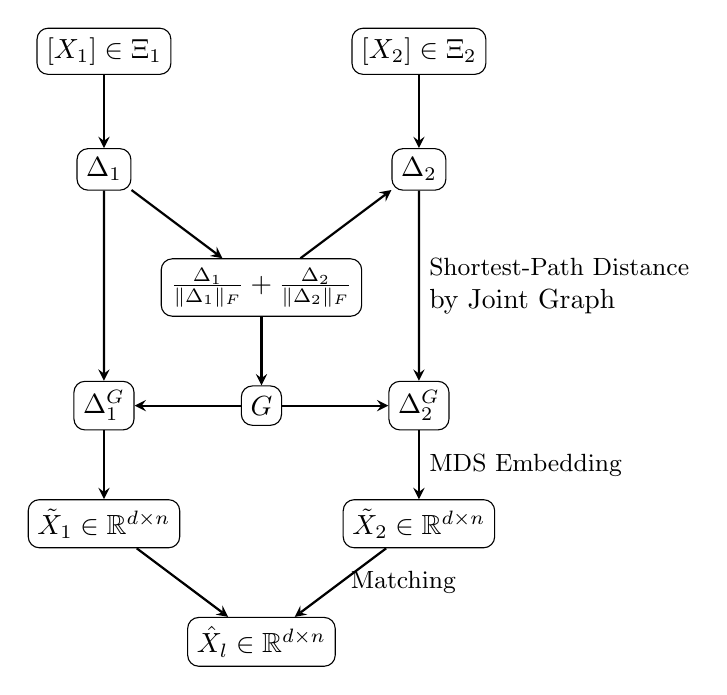
\begin{tikzpicture}[node distance=1.5cm]
\centering
%\node (in1) [node, yshift=0.5cm] {$X_{1} \in \Xi_{1}$};
%\node (in2) [node, yshift=-0.5cm] {$X_{2} \in \Xi_{2}$};
%\node (G) [node, right of=in1,yshift=-0.5cm] {$G$};
%\node (D1) [node, right of=G,yshift=0.5cm] {$\Delta_{1}^{G}$};
%\node (D2) [node, right of=G,yshift=-0.5cm] {$\Delta_{2}^{G}$};
%\node (end) [node, right of=D1,yshift=-0.5cm] {$\hat{X}_{l} \in \mathbb{R}^{d}$};
\node (in1) [node, xshift=4cm] {$[X_{1}] \in \Xi_{1}$};
\node (in2) [node, xshift=8cm] {$[X_{2}] \in \Xi_{2}$};
\node (D1) [node, below of=in1] {$\Delta_{1}$};
\node (D2) [node, below of=in2] {$\Delta_{2}$};

\node (D12) [node, below of=D1,xshift=2cm] {$\frac{\Delta_{1}}{\|\Delta_{1}\|_{F}}+\frac{\Delta_{2}}{\|\Delta_{2}\|_{F}}$};
\node (G) [node, below of=D12] {$G$};
\node (DG1) [node, left of=G,xshift=-0.5cm] {$\Delta_{1}^{G}$};
\node (DG2) [node, right of=G,xshift=0.5cm] {$\Delta_{2}^{G}$};
\node (X1) [node, below of=DG1] {$\tilde{X}_{1} \in \mathbb{R}^{d \times n}$};
\node (X2) [node, below of=DG2] {$\tilde{X}_{2} \in \mathbb{R}^{d \times n}$};
\node (end) [node, below of=X1,xshift=2cm] {$\hat{X}_{l} \in \mathbb{R}^{d \times n}$};

\draw [arrow] (in1) -- (D1);
\draw [arrow] (in2) -- (D2);
\draw [arrow] (D1) -- (D12);
%\draw [arrow] (D2) -- (D12);
\draw [arrow] (D12) -- (D2);
\draw [arrow] (D12) -- (G);
\draw [arrow] (D1) -- (DG1);
\draw [arrow, align=left] (D2) -- node[anchor=west] {\small Shortest-Path Distance \\ by Joint Graph}(DG2);
\draw [arrow] (G) -- (DG1);
\draw [arrow] (G) -- (DG2);
\draw [arrow] (DG1) -- (X1);
\draw [arrow] (DG2) -- node[anchor=west] {\small MDS Embedding}(X2);
\draw [arrow] (X1) -- (end);
\draw [arrow] (X2) -- node[anchor=west] {\small Matching}(end);
\end{tikzpicture}

\subsection{Implementation Details}
\label{discuss}
In this subsection, we discuss some implementation details of MMSJ, and the benchmarks we compare with.

The joint neighborhood graph ensures consistent neighborhood selection in the case of noisy or nonlinear modality, and is intuitively better than two separate neighborhood graphs for later matching when the correspondence are known. Alternatively, one may use a weighted sum of distances or rank-based method to derive the joint neighborhood graph instead. Note that it is necessary for the distance matrices to be properly scaled so that the joint neighborhood selection is meaningful, and joint neighborhood should not be used for unknown correspondence like the testing data. 

The shortest-path distance can recover the geodesic distance of isometric manifolds with high probability under certain sampling conditions \citep{BernsteinEtAl2000, SilvaTenenbaum2003}. When used together with joint neighborhood, the shortest-path distance makes use of the correspondence information. Computationally, the shortest-path distance matrix can be effectively implemented by Floyd's algorithm or Dijkstra's algorithm \citep{TenenbaumSilvaLangford2000}, which can be further sped up by choosing a small set of landmark points \citep{SilvaTenenbaum2003, BengioEtal2003}. For testing data, we essentially treats the training data as landmark points and only computes the shortest path distances from the testing to the training.

Embedding the shortest-path distance matrices followed by matching is a standard procedure. Alternatively, one may match the embeddings by CCA or joint MDS, as discussed in \citep{PriebeMarchette2012, FishkindShenPriebe2016}. The advantages of MMSJ mostly lie in joint neighborhood and shortest-path distance; in fact, MMSJ always exhibits significant improvement, no matter which matching method to use. Thus we mainly consider the Procrustes matching for ease of presentation in the paper. Note that the testing data are embedded by out-of-sample MDS, which is a standard technique for MDS and kernel PCA \citep{ScholkopfSmolaMuller1998,BengioEtal2003,TrossetPriebe2008}, and more efficient than re-embedding all training and testing data. After the testing data are mapped onto the manifolds by the learned Procrustes matching, we may test the matched-ness of any two testing observations from different data sources as in section~\ref{bg}.

To compare with MMSJ, we use the common procedure that embed each modality separately by MDS / Isomap / LLE / LTSA, followed by Procrustes matching. Note that MDS / Isomap / LLE can all operate directly on a distance matrix, but some nonlinear algorithms like LTSA have to start with the Euclidean data rather than a distance measure. Thus, if only the distance matrices are available, MDS is first used to embed the distance matrices into a Euclidean space $\mathbb{R}^{d'}$ with $d' \geq d$, followed by LTSA to embed into $\mathbb{R}^{d}$, then Procrustes matching.

\section{Numerical Experiments}
\label{numer}
In this section we demonstrate the numerical advantages of the proposed manifold matching algorithm, with MDS, Isomap, LLE, and LTSA as the benchmarks. Overall, we observe that our algorithm is significantly better than all the benchmarks in matching ratio and testing power. 

\subsection{Swiss Roll Simulation}
The Swiss roll data from \citep{TenenbaumSilvaLangford2000} is a 3D dataset representing a nonlinear manifold, but intrinsically generated by points on a 2D linear manifold. Figure~\ref{fig1} shows the 3D Swiss roll data with $5000$ points in colors, along with its 2D embeddings by MDS, Isomap, and LLE. Clearly, MDS fails to recognize the nonlinear geometry while both Isomap and LLE succeed. However, the LLE embedding has a distorted geometry, while the Isomap embedding is similar to the underlying 2D linear manifold.

\begin{figure}[htbp]
\centering
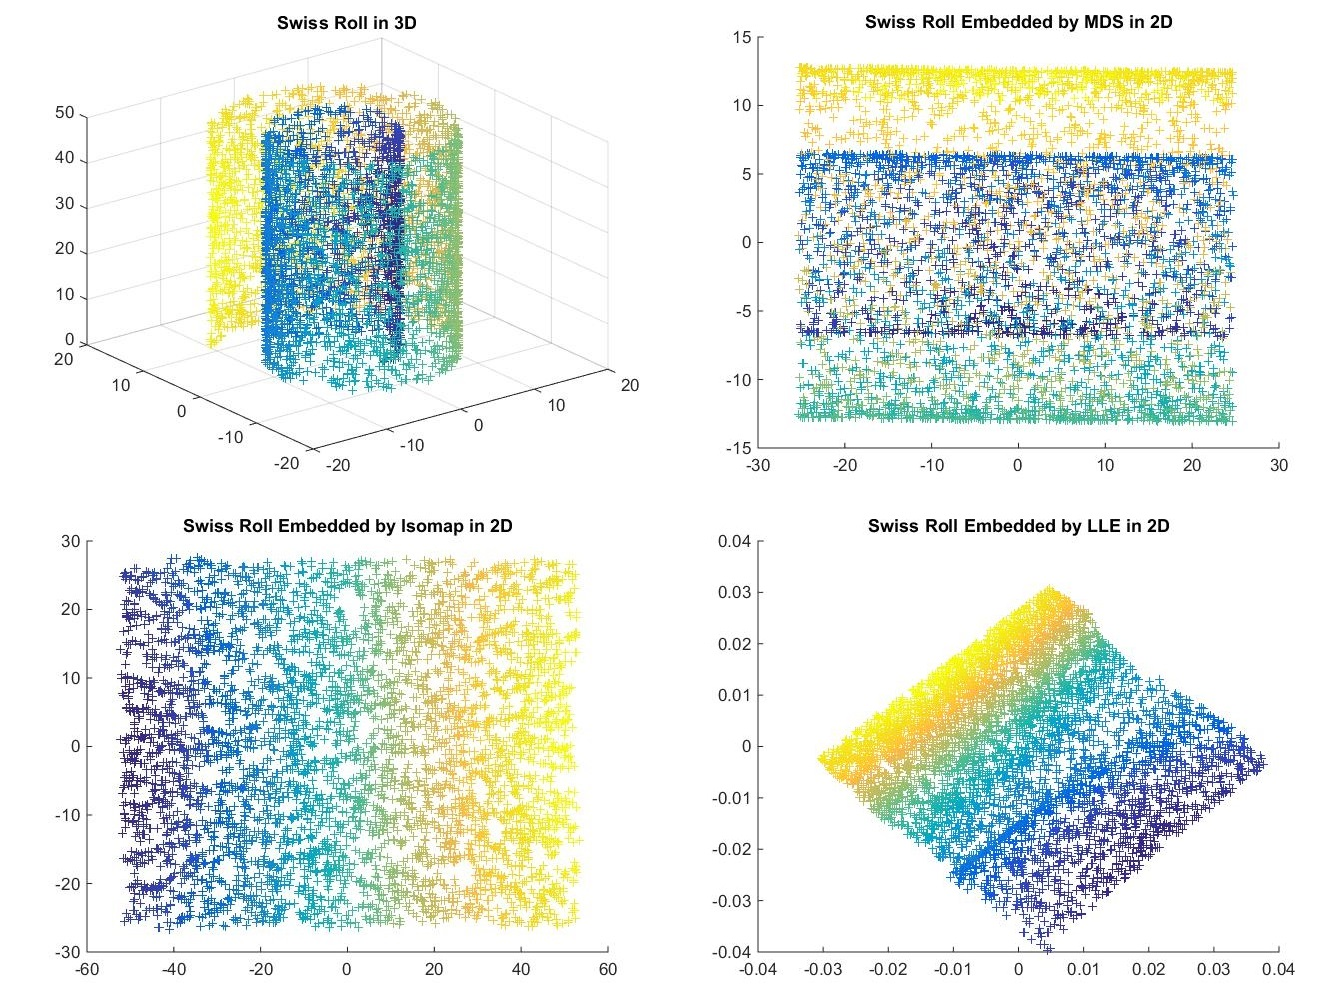
\includegraphics[width=0.5\textwidth]{../Figures/Swiss}
\caption{The 3D Swiss roll dataset (top left), its 2D embedded data by MDS (top right), 2D embedding by Isomap at neighborhood size $k=10$ (bottom left), and 2D embedding by LLE at $k=10$ (bottom right).}
\label{fig1}
\end{figure}

For the first simulation, we match the 3D Swiss roll with its underlying 2D linear manifold. A total of $n=1000$ points from the 3D Swiss roll are randomly generated to construct the first modality $X_{1}$, and the corresponding points on the underlying 2D linear manifold are taken as the second modality $X_{2}$. Thus $X_{1}$ and $X_{2}$ are matched training data with distinct geometries. Once the training data are matched, we embed and apply the learned mappings to new testing observations $y_{1}$ and $y_{2}$ in each space.

We set the neighborhood size as $k=10$ and the dimension choice as $d=2$, and use $100$ matched testing pairs and $100$ unmatched testing pairs to calculate the test statistic under the null and the alternative hypotheses. Repeat the above for $100$ Monte-Carlo replicates. The mean testing powers with respect to the increasing type $1$ error level are plotted in Figure~\ref{fig2}(a). The matching ratio is estimated based on the same $100$ matched testing pairs from $100$ MC replicates, which is shown in the first row of Table~\ref{table:Swiss}. The proposed MMSJ is clearly much better than all the benchmarks in both the testing power and the matching ratio. MDS and LTSA have the worst matching performance, while Isomap and LLE perform reasonably good.

Next, we check the robustness of the manifold matching algorithms against noise, by adding white noise to the linear modality $X_{2}$. The noise is independently and identically distributed as $Normal(0, \epsilon I_{2 \times 2})$, and the same testing procedure is applied to estimate the testing powers at each noise level. The powers are plotted in Figure~\ref{fig2}(b) with respect to the increasing noise level $\epsilon = 0,1,2,\ldots,10$ at type $1$ error level $0.05$. The proposed MMSJ algorithm is still better than all the benchmarks as the noise level increases.

For the third simulation, we match two linear modalities: instead of the 3D Swiss roll, we use the 2D LLE embedding as $X_{1}$; thus $X_{1}$ and $X_{2}$ are both linear with some differences. Using the same procedure and parameters as the first simulation, the testing power is plotted in Figure~\ref{fig2}(d) and the matching ratio is shown in the second row of Table~\ref{table:Swiss}. In this case MMSJ, MDS, and Isomap have similar performances with LLE and LTSA being slightly worse, which indicates that the shortest-path distance is more robust when matching noisy linear manifolds. Note that the matching ratio and testing power here are lower than those in the first simulation, because the LLE embedding has a distorted linear geometry. 

\begin{table*}[htbp]
\centering
\caption{Swiss Roll Matching Ratio}
\label{table:Swiss}
\begin{tabular}{|c||c|c|c|c|c|}
\hline
Modalities & MMSJ & MDS & Isomap & LLE & LTSA \\
\hline
$(\mbox{3D Swiss Roll}, \mbox{2D Linear Manifold})$ & $\textbf{0.9787}$  & $0.0200$ & $0.1324$ & $0.2123$ & $0.0697$\\
\hline
$(\mbox{2D LLE Embedding}, \mbox{2D Linear Manifold})$ & $\textbf{0.1771}$  & $0.1386$ & $0.1412$ & $0.1248$ & $0.0828$\\
\hline
\end{tabular}
\end{table*}

\subsection{Wikipedia Articles Experiments}
In the real data experiments, we apply the manifold matching algorithm to match disparate features of Wikipedia articles. The raw data contains $1382$ pairs of articles from Wikipedia English and its corresponding French translations, within the 2-neighborhood of the English article ``Algebraic Geometry". On Wikipedia, the same articles of different languages are almost never the exact translations of each other, because they are very likely written by different people and their contents may differ in many ways.

For the English articles and their French translations, a text feature and a graph feature are collected separately under each language. For the texts of each article, we use latent semantic indexing (LSI) \citep{DeerwesterDumais1990} followed by cosine dissimilarity to construct two dissimilarity matrices $TE$ and $TF$ (representing the English texts and French texts). For the networks, two shortest-path distance matrices $GE$ and $GF$ (representing the English graph and French graph) are calculated based on the Internet hyperlinks of the articles under each language setting, with any path distance larger than $4$ imputed to be $6$ to avoid infinite distances and scaling issues.

Therefore, there exist four different modalities for the same Wikipedia articles, making $TE$, $TF$, $GE$, and $GF$ matched in the context. Furthermore, as the text matrices are derived by cosine similarity while the graph matrices are based on the shortest-path distance with imputation, the former probably have nonlinear geometries while the latter are linear from the view of our matching algorithm.

For each Monte-Carlo replicate, we randomly pick $n=500$ pairs of training observations, $100$ pairs of testing matched observations, and $100$ pairs of testing unmatched observations for evaluation. The parameters are set as $k=20$, $d=10$, $d'=50$ (for LTSA only), and the manifold matching algorithms are applied for every possible combination of matching two modalities. After $100$ Monte-Carlo replicates, the mean matching ratio is reported in Table~\ref{table:wikiAcc}, the estimated testing power is presented in Table~\ref{table:wikiPower} at type $1$ error level $0.05$, and the power curves for some matching combinations are plotted in Figure~\ref{figReal}. 

Clearly, MMSJ achieves the best performance throughout all combinations. From the tables and figures, we further observe that without using shortest-path distance or joint neighborhood, separate nonlinear embeddings from LLE or LTSA are worse than the linear MDS embeddings in matching. Isomap does fairly well in the testing power, as it also uses shortest-path distance, but it can still be similar or slightly inferior to MDS in the matching ratio occasionally. Our proposed MMSJ algorithm is consistently the best manifold matching algorithm in both the testing power and the matching ratio throughout.

We should point out that the matching performance depends on the parameters $k$ and $d$, and the testing power or matching ratio of each algorithm can be slightly different by changing the parameters. For example, the MDS testing power is $0.49$ for matching $(TE, TF)$ at $d=10$, which can be improved to $0.7$ by varying $d$. MMSJ has the best power of $0.82$, which can be increased to $0.9$ by cross-validating the parameters as well. So far we have used fixed parameter choices to offer meaningful comparisons throughout all algorithms and matching combinations, but our MMSJ algorithm is in fact robust against misspecification of parameters. As an example, in Figure~\ref{figRealSurf} we show the MMSJ and Isomap testing powers for matching $(TE,GE)$ (the best two algorithms in our matching experiments) against different choices of $d$ and $k$, for which $d$ ranges from $2$ to $30$ and $k$ ranges from $10$ to $30$. It is clear that MMSJ is always better than Isomap in matching and attains close-to-optimal testing power in a large range of parameter choices. Furthermore, the best MMSJ testing power is $0.55$ while the best Isomap testing power is $0.45$. The same robustness holds for MMSJ under all other matching combinations. 

%Note that choosing $k$ and $d$ for the Swiss roll data is quite easy, because the neighborhood size has been validated by many previous works and the embedding dimension should equal the intrinsic true dimension. But for real data experiments, the parameter choice is usually dependent on the later inference task.

\begin{Table}
\centering
\captionof{table}{Wikipedia Features Matching Ratio}
\label{table:wikiAcc}%
\begin{tabular}{|c||c|c|c|c|c|}
\hline
Modalities & MMSJ & MDS & Isomap & LLE & LTSA \\
\hline
$(TE, TF)$ & $\textbf{0.2942}$  & $0.2546$ & $0.2003$ & $0.1265$ & $0.0491$\\
\hline
$(TE, GE)$ & $\textbf{0.1209}$  & $0.0675$ & $0.0866$ & $0.0143$ & $0.0260$\\
\hline
$(TF, GF)$ & $\textbf{0.0624}$  & $0.0419$ & $0.0522$ & $0.0134$ & $0.0144$\\
\hline
$(GE, GF)$ & $\textbf{0.1347}$  & $0.1280$ & $0.1081$ & $0.0157$ & $0.236$\\
\hline
$(TE, GF)$ & $\textbf{0.0677}$  & $0.0429$ & $0.0560$ & $0.0132$ & $0.0138$\\
\hline
$(TF, GE)$ & $\textbf{0.0946}$  & $0.0545$ & $0.0698$ & $0.0132$ & $0.0238$\\
\hline
\end{tabular}
\end{Table}

\begin{Table}
\centering
\captionof{table}{Wikipedia Features Testing Power at Type $1$ Error Level 0.05}
\label{table:wikiPower}
\begin{tabular}{|c||c|c|c|c|c|}
\hline
Modalities & MMSJ & MDS & Isomap & LLE & LTSA \\
\hline
$(TE, TF)$ & $\textbf{0.8124}$  & $0.4974$ & $0.7476$ & $0.3594$ & $0.1930$\\
\hline
$(TE, GE)$ & $\textbf{0.5184}$  & $0.2563$ & $0.4255$ & $0.0948$ & $0.1116$\\
\hline
$(TF, GF)$ & $\textbf{0.2782}$  & $0.1128$ & $0.1877$ & $0.0903$ & $0.1028$\\
\hline
$(GE, GF)$ & $\textbf{0.3108}$  & $0.2141$ & $0.2485$ & $0.0961$ & $0.1063$\\
\hline
$(TE, GF)$ & $\textbf{0.3199}$  & $0.1130$ & $0.2141$ & $0.0923$ & $0.1021$\\
\hline
$(TF, GE)$ & $\textbf{0.4464}$  & $0.2114$ & $0.3595$ & $0.0943$ & $0.1064$\\
\hline
\end{tabular}
\end{Table}

\begin{figure*}
  \centering
  \begin{tabular}{@{}p{\linewidth}@{\quad}p{\linewidth}@{}}
	\centering
    \subfigimg[width=0.32\linewidth]{A}{../Figures/SwissRoll1}
    \subfigimg[width=0.32\linewidth]{B}{../Figures/SwissRoll1Noise}
    \subfigimg[width=0.32\linewidth]{C}{../Figures/SwissRoll2}
  \end{tabular}
  \caption{ Testing Powers of Swiss Roll Datasets with respect to Increasing Type $1$ Error Level.
(A) Testing Power of 3D Swiss Roll versus its 2D Underlying Linear Manifold.
(B) Testing Power of 3D Swiss Roll versus its 2D Underlying Linear Manifold with Increasing Noise.
(C) Testing Power of 2D LLE Embedding of Swiss Roll versus its 2D Underlying Linear Manifold. }
\label{fig2}
\end{figure*}

\begin{figure*}
  \centering
  \begin{tabular}{@{}p{\linewidth}@{\quad}p{\linewidth}@{}}
	\centering
    \subfigimg[width=0.32\linewidth]{A}{../Figures/WikiTETF}
    \subfigimg[width=0.32\linewidth]{B}{../Figures/WikiTEGE}
    \subfigimg[width=0.32\linewidth]{C}{../Figures/WikiGEGF}
  \end{tabular}
  \caption{Testing Powers of Wikipedia Datasets with respect to Increasing Type $1$ Error Level.
(A) Testing Power of Wikipedia English Text versus French Text.
(B) Testing Power of Wikipedia English Text versus English Graph.
(C) Testing Power of Wikipedia English Graph versus French Graph.}
\label{figReal}
\end{figure*}

\begin{figure*}
  \centering
  \begin{tabular}{@{}p{\linewidth}@{\quad}p{\linewidth}@{}}
	\centering
    \subfigimg[width=0.4\linewidth]{A}{../Figures/WikiTEGESurf1}
    \subfigimg[width=0.4\linewidth]{B}{../Figures/WikiTEGESurf2}
  \end{tabular}
\caption{Testing Power of Wikipedia English Text and English Graph with respect to Different Dimension Choices and Neighborhood Sizes at Type $1$ Error Level 0.05.
(A) The testing power of MMSJ. (B) The testing power of Isomap.
}
\label{figRealSurf}
\end{figure*}

\section{Concluding Remarks}
\label{conclu}
In summary, we propose a nonlinear manifold matching algorithm using shortest-path distance and joint neighborhood selection. The algorithm is straightforward to implement, and achieves superior and robust performance. It is able to significantly improve the testing power and matching ratio when matching modalities of distinct geometries, and is robust against noise and model selection. Our experiments indicate that the shortest-path distance and joint neighborhood selection are two key catalysts behind the improvement of the matching performance.

Furthermore, the improvement in manifold matching motivates our follow-up work \citep{ShenEtAl2016} regarding dependency discovery by local scale, which makes use of the joint neighborhood and local distances in a similar manner.

\section*{Acknowledgment}
\addcontentsline{toc}{section}{Acknowledgment}
This work is partially supported by National Security Science and Engineering Faculty Fellowship (NSSEFF),
 Johns Hopkins University Human Language Technology Center of Excellence (JHU HLT COE), and the
 XDATA program of the Defense Advanced Research Projects Agency (DARPA) administered through Air Force Research Laboratory contract FA8750-12-2-0303. This work is also supported by the Defense Advanced Research Projects Agency (DARPA) SIMPLEX program through SPAWAR contract N66001-15-C-4041 and DARPA GRAPHS N66001-14-1-4028.

\bibliographystyle{model2-names}
\bibliography{references}

%\newpage 

%\section*{Supplementary Material}

\end{document}